\begin{flushright} {\tiny {\color{gray} fdm\_advdiff1D.tex}} \end{flushright}
%~~~~~~~~~~~~~~~~~~~~~~~~~~~~~~~~~~~~~~~~~~~~~~~~~~~~~~~~~~~~~~~~~~~~~~~~~~~~~~~~~~~~~~~~~~~~~~~~~~

The 1d advection-diffusion equation is:
\begin{equation}
\rho C_p \left( \frac{\partial T}{\partial t}  
+ u \frac{\partial T}{\partial x} \right)= k \frac{\partial^2 T}{\partial x^2} + H'
\end{equation}
or simply
\begin{equation}
\frac{\partial T}{\partial t} + u \frac{\partial T}{\partial x}= \kappa \frac{\partial^2 T}{\partial x^2} + H
\end{equation}
where $H=H'/\rho C_p$ is a source term that does not depend on time.
We have seen how to deal with the time derivative (explicit, implicit) 
and with the first order space derivative (forward, backward or central).
Let us consider the FTCS scheme (Forward in Time, Central in Space).
\[
\frac{T_{\color{teal}i}^{n+1}-T^n_{\color{teal}i}}{\delta t} 
+ u_i \frac{T^n_{\color{teal}i+1} - T^n_{{\color{teal}i-1}}}{2h} = \kappa \frac{T_{i+1}^n-2T_i^n+T_{i-1}^n}{h^2} + H_i
\]
Likewise we can consider the BTCS scheme:
\[
\frac{T_{\color{teal}i}^{n+1}-T^n_{\color{teal}i}}{\delta t} 
+ u_i \frac{T^{n+1}_{\color{teal}i+1} - T^{n+1}_{{\color{teal}i-1}}}{2h} 
= \kappa \frac{T_{i+1}^{n+1}-2T_i^{n+1}+T_{i-1}^{n+1}}{h^2} + H_i
\]
which makes the method implicit. 
Or, using a Crank-Nicolson approach:
\[
\frac{T_{\color{teal}i}^{n+1}-T^n_{\color{teal}i}}{\delta t} 
=
\frac12
\left(
- u_i \frac{T^{n+1}n_{\color{teal}i+1} - T^{n+1}_{{\color{teal}i-1}}}{2h} 
+ \kappa \frac{T_{i+1}^{n+1}-2T_i^{n+1}+T_{i-1}^{n+1}}{h^2} 
- u_i \frac{T^n_{\color{teal}i+1} - T^n_{{\color{teal}i-1}}}{2h} + \kappa \frac{T_{i+1}^n-2T_i^n+T_{i-1}^n}{h^2} 
\right)
+ H_i
\]




As we have seen before, the advection term is a source of problems and multiple 
methods have been designed to stabilise the pure advection equation. 
The {\color{olive}Fiadeiro \& Veronis method} \cite{five77,wrig92}, works as follows for the (steady state)
advection-diffusion equation (see also p315 of \textcite{boudreau}):
\[
\kappa \frac{T_{i+1}-2T_i + T_{i-1}}{h^2}
- u \frac{(1-\sigma) T_{i+1}+2\sigma T_i -(1+\sigma)T_{i-1}}{2 h} = 0
\]
which is a blend of backward (upstream) and central differences. The amount of
blending is dictated by the value of the parameter $\sigma$, defined as
\[
\sigma 
= \text{coth} \frac{u h}{2 \kappa} - \frac{2 \kappa}{u h}
= \text{coth} \; \Penb  - \frac{1}{\Penb}
\]
The parameter $\sigma$ has the property that
$\sigma \rightarrow 0$ when $\Penb \rightarrow 0$ and 
$\sigma \rightarrow 1$ when $\Penb \rightarrow \infty$.
The equation above can also be rewritten:
\[
\kappa \frac{T_{i+1}-2T_i + T_{i-1}}{h^2}
- u \frac{1 T_{i+1}-T_{i-1}}{2 h} = 0
+ \frac{u \sigma h}{2} \frac{T_{i+1}-2 T_i +T_{i-1}}{h^2} = 0
\]
which makes the action of this stabilisation term more obvious: it is a diffusion term whose 
diffusion coefficient goes away when $h\rightarrow 0$. 

Thus, if $\sigma = 0$ (diffusion dominated), then pure central differencing is obtained, and if
$\sigma = 1$ (advection dominated), then pure backward differencing results. Interestingly
enough, this blended or weighted scheme is second-order accurate even as it switches
to backward differencing \cite{five77}. 
Note that it is essentially the known streamline upwind method used in FEM or FDM (see
Section~\ref{ss:fdm_adv1D}). 
Also, when $\kappa \rightarrow 0$ (no physical diffusion at all)
then $\sigma$ tends to $\pm 1$, and more precisely: $\sigma = sign(u)$, which allows for a simple 
and elegant implementation. 

Adding a FT time derivative term, the equation above can be rewritten (a source
term has been added):
\[
\frac{T_{\color{teal}i}^{n+1}-T^n_{\color{teal}i}}{\delta t} 
=
\kappa \frac{T_{i+1}^n-2T_i + T_{i-1}^n}{h^2}
- u \frac{(1-\sigma) T_{i+1}^n+2\sigma T_i^n -(1+\sigma)T_{i-1}^n}{2 h} +H 
\]



\paragraph{A simple example} Let us consider the domain $0<x<1$.
Let us prescribe $T(x=0)=0$  and $T(x=1)=0$ and we want to solve 
the steady state advection diffusion equation (with a source term):
\begin{equation}
u \frac{\partial T}{\partial x} = \kappa \frac{\partial^2 T}{\partial x^2} + 1
\label{eq:fdmadvdiff2}
\end{equation}
The solution is then 
\begin{equation}
T(x)=x - \frac{\exp (-(1-x)/\kappa) -\exp (-1/\kappa)  }{1-\exp (-1/\kappa)}
\label{eq:fdmadvdiff1}
\end{equation}

In this case, if $u\rightarrow 0$ then the equation becomes a diffusion equation
and the solution is $T(x)=0$. If $u$ is large, the field is advected to the right
but the right boundary condition $T(x=1)=0$ poses a problem which results in a very steep slope
and potentially numerical issues too for the FTCS method, but not for the FTFV method.

\begin{center}
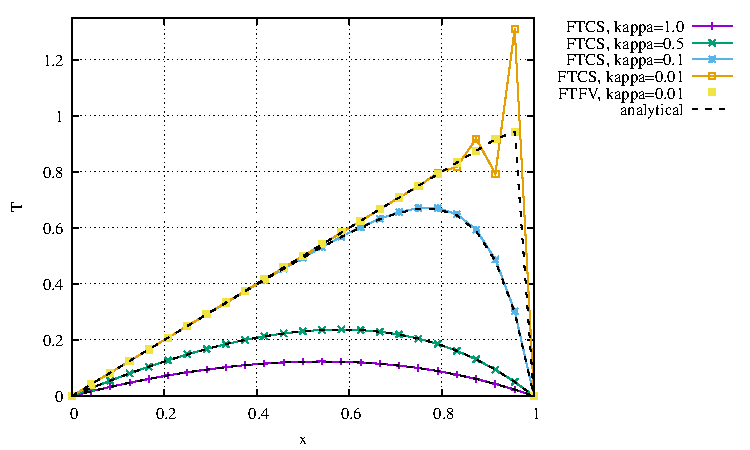
\includegraphics[width=11cm]{images/fdm/adv_diff/T.pdf}\\
{\captionfont Results obtained with FTCS method. nnx=25, $u=1$, $\delta t=10^{-4}$, 
nstep=25000. FTFV stands for 'forward in time, Fiadeiro \& Veronis'}
\end{center}

A very similar example is implemented in \stone~65 (albeit with FEM).

%-/-/-/-/-/-/-/-/-/-/-/-/-/-/-/-/-/-/-/
\begin{center}
\begin{minipage}[t]{0.77\textwidth}
\par\noindent\rule{\textwidth}{0.4pt}

\begin{center}
\includegraphics[width=0.8cm]{images/garftr} \\
{\color{orange}Exercise FDM-8}
\end{center}

Prove that Eq.~\eqref{eq:fdmadvdiff1} is indeed solution of 
Eq.~\eqref{eq:fdmadvdiff2}. Code the FTCS and FTFV methods and reproduce 
the figure above (i.e. only forward in time/explicit methods).

\par\noindent\rule{\textwidth}{0.4pt}
\end{minipage}
\end{center}
%-/-/-/-/-/-/-/-/-/-/-/-/-/-/-/-/-/-/

